\documentclass{article}

\usepackage{xcolor,listings,amsthm,amssymb,amsmath}
\usepackage{graphicx}
\usepackage[backend=biber, style=mla, citestyle=authoryear]{biblatex}
\usepackage{euler}

\usepackage[shortlabels]{enumitem}
\usepackage[utf8]{inputenc}
\usepackage[english]{babel}

\addbibresource{project.bib}
\graphicspath{ {./images/} }

\author{Rohit Wason}
\newtheorem{problem}{Problem}
\newtheorem*{solution*}{Solution}
\renewcommand{\theenumi}{\alph{enumi}\)}

\title{MATH 560 - Project}
\date{4/19/2021}

\begin{document}
\maketitle

\section*{Abstract}
According to the World Health Organization (WHO) stroke is the 2nd leading cause of death globally, 
responsible for approximately 11\% of total deaths. This dataset is used to predict whether a patient
is likely to get stroke based on the input parameters like gender, age, various diseases, and smoking 
status. Here we use a public dataset of patients to state hypotheses of correlation between various explanatory
variables (like, age, bmi, marital status, residence type, etc.) along with the fact that they have had
a stroke.\\
\pagebreak

\section*{The Dataset}
The dataset we use here can be found on Kaggle, a public competetion forum
where data scientists and novices collaborate to find answers in complex datasets
(\cite{kaggle}). This dataset contains $5110$ data points with $12$ variables:
\begin{itemize}
  \item \textbf{id}
    \textsubscript{Unique Identifier. (We will ignore this variable, as we're not interested in the individual patient's details)}
  \item \textbf{gender}
    \textsubscript{("Male", "Female" or "Other")}
  \item \textbf{age}
    \textsubscript{(Age of the patient)}
  \item \textbf{hypertension}
    \textsubscript{(0 if the patient doesn't have hypertension, 1 if the patient has hypertension)}
  \item \textbf{heart\_disease} 
    \textsubscript{(0 if the patient doesn't have any heart diseases, 1 if the patient has a heart disease)}
  \item \textbf{ever\_married} 
    \textsubscript{(``No'' or ``Yes'')}
  \item \textbf{work\_type} 
    \textsubscript{(``children'', ``Govt\_jov'', ``Never\_worked'', ``Private'' or ``Self-employed'')}
  \item \textbf{Residence\_type} 
    \textsubscript{(``Rural'' or ``Urban'')}
  \item \textbf{avg\_glucose\_level} 
    \textsubscript{(Average Glucose level in blood)}
  \item \textbf{bmi} 
    \textsubscript{(Body Aass Index)}
  \item \textbf{smoking\_status} 
    \textsubscript{(``formerly smoked'', ``never smoked'', ``smokes'' or ``Unknown'')}
  \item \textbf{stroke} 
    \textsubscript{(1 if the patient had a stroke or 0 if not)}
\end{itemize}
\pagebreak

\section*{Data Preparation}
As is usually the case with real data, there are inconsistencies in this dataset.
For example, \textit{numerical} variables, like ``bmi'' could be classified 
as \textit{categorical}. Such inconsistencies can hamper our research, 
hence are cleaned-up as a first step:\\

We start with analysing the ``class'' of each variable:\\

\begin{tabular}{l|l}\hline
  Variable & Class \\\hline
  id                  & Integer\\
  gender              & Categorical\\
  age                 & Numeric\\
  hypertension        & Integer\\
  heart\_disease      & Integer\\
  ever\_married       & Categorical\\
  work\_type          & Categorical\\
  Residence\_type     & Categorical\\
  avg\_glucose\_level & Numeric\\
  bmi                 & Categorical\\
  smoking\_status     & Categorical\\
  stroke              & Integer
\end{tabular}\\

We note that the ``bmi'' variable is classified as ``categorical''
because there are values like ``N/A'' for some items. We filter those out:
\begin{lstlisting}[backgroundcolor = \color{lightgray},language = R]
  > stroke=stroke[stroke$bmi!='N/A',]
  > stroke=transform(stroke, bmi=as.numeric(bmi))
  > dim(stroke)
  [1] 4909   12
\end{lstlisting}
As a result, out of $5110$ data-points, only $4909$ are 
rendered ``useful''. We consider this enough data for our research
and mark the interesting ``numeric'' variables:
\textbf{age}, \textbf{bmi} and \textbf{average\_glucose\_level}.
\pagebreak

\section*{The Analysis}
According to stroke.org, a non-profit organization dedicated to public awareness about,
and prevention of common causes of stroke, smoking, lack of physical activity, diabetes and 
obesity are leading factors that could lead to stroke (\cite{strokeorg}). An important
question to analyze would be ``Can we predict 
the onset of stroke given any/all of the variables in this dataset?''\\

However, since ``stroke'' is a ``categorical'' variable, and we want to limit our research 
to ``numeric'' values only, we explore the question:\\

\fbox{Is ``bmi'' correlated to any other ``numeric'' value?}\\

It is customary while analyzing data, to ``slice and dice''
data in different ways. One such way is to find correlated 
variables, so their presence doesn't falsly influence the 
dependent variable. Therefore, while it might be possible 
to answer more important questions using this data, 
the present question is of some value in the big picture.
\pagebreak

At this point we plot ``bmi'' against other ``numeric'' variables.
As a convention, the independent variable is shown horizontally
(on the \textbf{x-axis}), and the dependent variable,
vertically (on the \textbf{y-axis}).\\
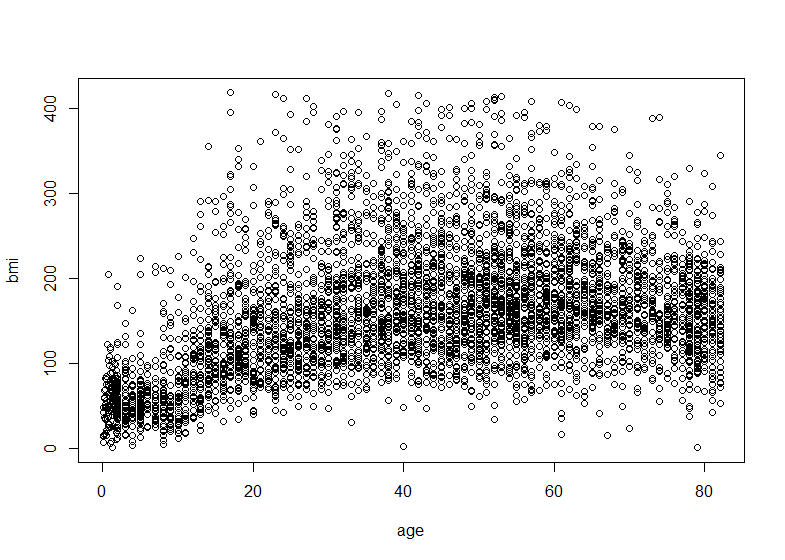
\includegraphics[scale=.5]{bmi-age}\\
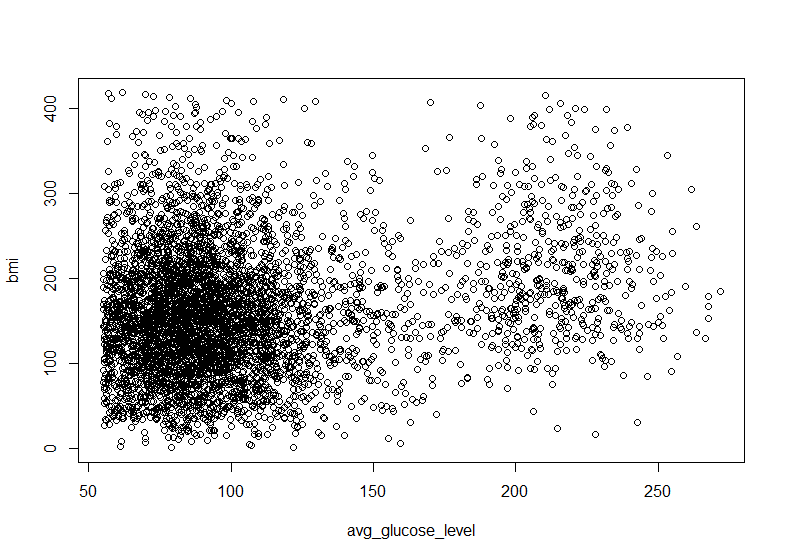
\includegraphics[scale=.5]{bmi-avg_glucose_level}\\

Graphically, there seems to be some correlation between ``bmi''
and each of the ``average\_glucose\_level'' and ``age''. It seems plausible
that the latter two variables, also known as \textbf{independent variables}
could affect the former, the \textbf{dependent variable}.
\pagebreak

\section*{Data Modelling}
The technique of Linear Regression is common in research of this type
– the dependent variable (``bmi'', in this case) can be modelled
with the independent ones. This technique is called ``fitting'',
and results in a linear equation involving all the variables
involved of the kind

\begin{equation}
  \hat{y} = \beta_0 + \beta_1(x_1) + \beta_2(x_2) + \dots + \beta_p(x_p)
\end{equation}

where $\beta_i$ are called the \textbf{regression coefficients} 
corresponding to the \textbf{independent variables}, $x_i$
($i=1,2,3,\dots,p$).\\

The \textbf{R programming language} offers a powerful way to ``fit''
this model:

\begin{lstlisting}[backgroundcolor = \color{lightgray},language = R]
  > lmStroke=lm(bmi~age+avg_glucose_level, data=stroke)
\end{lstlisting}

What this created is a ``linear model'' called ``lmStroke''
using the 3 interesting variables, for the $4909$ data-points.
The model could be seen as a projected line in a 3-dimensional
space (a dimention representing each of the variables we're 
interested in). And what's fascinating is that these models 
do not have to be limited to 3-dimentional space only.
Most real-data consist of hundreds, or thousands of variables
and can be ``fitted'' in the same way our model is!\\

We now observe the summary of this model:
\begin{lstlisting}[backgroundcolor = \color{lightgray},language = R]
  Coefficients:
                    Estimate Std. Error t value Pr(>|t|)    
  (Intercept)       96.90234    2.91577  33.234  < 2e-16
  age                1.08004    0.04556  23.705  < 2e-16
  avg_glucose_level  0.17939    0.02313   7.755 1.07e-14
\end{lstlisting}

One important characteristic of this model is the 
coefficients ($\beta_i$) for each independent variable.
Using the specific values of this model
we get our version of equation ($1$) above
as:

\begin{equation}
  \hat{y} = 96.9023 + 1.0800(x_1) + 0.1793(x_2)
\end{equation}

which is powerful, since if the independent
variables, ``age'' and ``avg\_glucose\_level''
($x_1, x_2$ here) correlate with the independent variable,
``bmi'', they can be used to predict ``bmi'' ($\hat{y}$
is the predicted value of $y$).

\subsection*{ANOVA F-test}
An important analysis of this model is called Analysis of variance (ANOVA).
It can determine whether the means of three or more groups are different. 
ANOVA uses \textbf{F-tests} to statistically test the equality of means.\\

The reason this analysis is important is to statistically rate variables
on their ``importance'' in predicting the independent variable.

\subsection*{Hypotheses}
We test the \textbf{null hypothesis}, $H_0$ that 
all independent variables are insignificant in determining
the dependent variables. In other words, their coefficients 
$\beta_1=\beta_2=0$. This is tested against the alternative
hypothesis, $H_a$ that such is not the case.

\begin{lstlisting}[backgroundcolor = \color{lightgray},language = R]
  Residuals:
      Min      1Q  Median      3Q     Max 
  -194.40  -49.45  -13.30   35.90  291.67 

  Residual standard error: 69.96 on 4906 DF
  Multiple R-squared:0.1327, Adjusted R-squared:0.1323 
  F-statistic: 375.2 on 2 and 4906 DF,  p-value:<2.2e-16
\end{lstlisting}

On examining the above summary of our model, we see
that the test statistic
$$F=\frac{MSM}{MSE}=375.2,$$
which when compared to
$$f^*=39.4$$
is much greater. Hence we \textbf{reject}
the hypothesis that 
all independent variables are insignificant in determining
the dependent variables. In other words, the independent
variables, ``age'' and ``average\_glucose\_level'' cannot be 
discarded as playing a role in determining ``bmi''.

\pagebreak

\section*{Summary}
We started with examining a health-related dataset from the 
public domain. We also started with the assumption
that the data collection is unbiased and fair.\\
After an initial cleanup of some anomalies, the data
seemed fairly useful with the ``numeric'' variables.
Especially of interest were the ``bmi'', ``age''
and ``average\_glucose\_level'' variables and we grew 
interested in finding if these variables exhibit any correlation.\\
On regressing the latter two variables to ``fit'' the value of 
``bmi'', we observe that the correlation is significant
and that \textbf{the two independent variables 
cannot be discarded, while predicting the ``bmi''.}
\pagebreak

\printbibliography

\end{document}
